\section{Аналитическая часть}

В данном разделе рассмотрены существующие решения, формализована задача и данные, выделены категории пользователей, а также выбрана модель базы данных.

\subsection{Существующие решения}

В связи с существованием потребности в системах планирования, на рынке уже существуют решения, предоставляющие различный функционал.

Рассмотрим только самые популярные из них, такие как:
\begin{itemize}[]
	\item Яндекс.Календарь;
	\item календарь Outlook;
	\item календарь Google.
\end{itemize}

Выделим следующие критерии для сравнения выбранных решений.
\begin{enumerate}[]
	\item Возможность приглашать с событиям участников.
	\item Возможность гибкой настройки прав доступа для каждого участника.
	\item Возможность добавлять теги.
	\item Возможность гибкого поиска событий.
\end{enumerate}

Результаты сравнения выбранных решений по заданным критериям представлены в таблице \ref{tbl:exist}.

\begin{table}[ht!]
	\centering
	\caption{Существующие решения поставленной задачи}
	\label{tbl:exist}
	\begin{tabular}{|p{2.6cm}|p{3cm}|p{4cm}|p{3cm}|p{2cm}|}
		\hline
		\textbf{Название проекта}         & \textbf{Возм. приглашать участников} & \textbf{Возм. настройки прав доступа} & \textbf{Возм. добавлять теги} & \textbf{Возм. гибкого поиска событий} \\ \hline
		\textbf{Яндекс. Календарь} \cite{yandex}   &  Да                                   & Только для всех участников сразу                                    & Нет                             &  Нет                                     \\ \hline
		\textbf{Календарь Outlook} \cite{outlook}   & Да                                    & Нет                                      & Да                             & Да                                      \\ \hline
		\textbf{Календарь Google} \cite{google} & Да                                    & Только для всех участников сразу -                                     & Нет                             &   Да                                    \\ \hline
	\end{tabular}
\end{table}

Таким образом, ни одно из четырех рассмотренных решений не удовлетворяет всем четырем критериям сравнения. Также стоит отметить, что ни в одной из рассмотренных систем нет возможности назначать права доступа к событию индивидуально для каждого приглашенного пользователя.

\subsection{Формализация задачи}

В ходе выполнения курсовой работы необходимо разработать базу данных для хранения информации о пользователях, событиях, приглашениях, правах доступа и тегах. Также необходимо спроектировать и разработать приложение, которое будет предоставлять API-интерфейс для взаимодействия с базой данных. 

Необходимо предусмотреть возможность создавать события с указанием названия, временной метки, описания, типа,  тегов и приглашенных пользователей. Реализовать возможность для приглашенного пользователя просматривать, менять событие или приглашать других участников в зависимости от выданных ему прав доступа к событию. Помимо этого, требуется реализовать возможность фильтрации и сортировки по различным данным события.

\subsection{Формализация данных}

В разрабатываемой базе данных можно выделить следующие сущности:

\begin{enumerate}[label=\arabic*.]
	\item пользователь --- User;
	\item событие --- Event;
	\item приглашение --- Invitation;
	\item право доступа --- Access Right;
	\item тег --- Tag.
\end{enumerate}

На рисунке \ref{fig:ER} представлена ER-диаграмма сущностей в нотации Чена.

\begin{figure}[ht!]
	\centering
	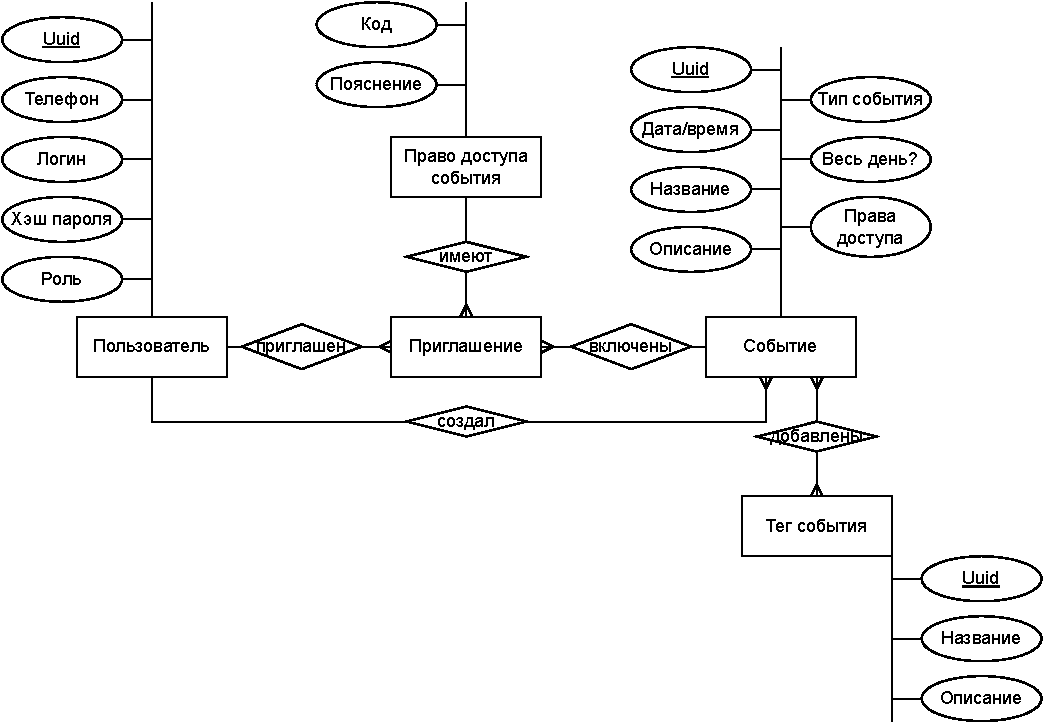
\includegraphics[width=0.9\linewidth]{assets/images/ER.pdf}
	\caption{ER-диаграмма в нотации Чена}
	\label{fig:ER}
\end{figure}
\FloatBarrier

\subsection{Формализация категорий пользователя}

Для взаимодействия с приложением было выделено 3 следующие категории пользователей.
\begin{enumerate}[label=\arabic*.]
	\item \textbf{Обычный пользователь} после входа в приложение может только создавать, изменять и удалять события и изменять данные своего пользователя.
	\item \textbf{Премиум пользователь} после входа в приложение может создавать, изменять и удалять события, изменять данные своего пользователя, а также производить поиск событий с фильтрацией, сортировкой и пагинацией.
	\item \textbf{Администратор} после входа в приложение может создавать, изменять и удалять события и теги, производить поиск событий с фильтрацией, сортировкой и пагинацией, а также изменять и удалять любых пользователей.
\end{enumerate}

Более того, доступ конкретного пользователя к событиям ограничивается указанными для него правами доступа при приглашении. Тем не менее, у администратора есть доступ к любым созданным событиям.

На рисунках \ref{fig:use-case-simple} -- \ref{fig:use-case-admin} представлены диаграммы вариантов использования приложения для каждой категории пользователей.

\begin{figure}[ht!]
	\centering
	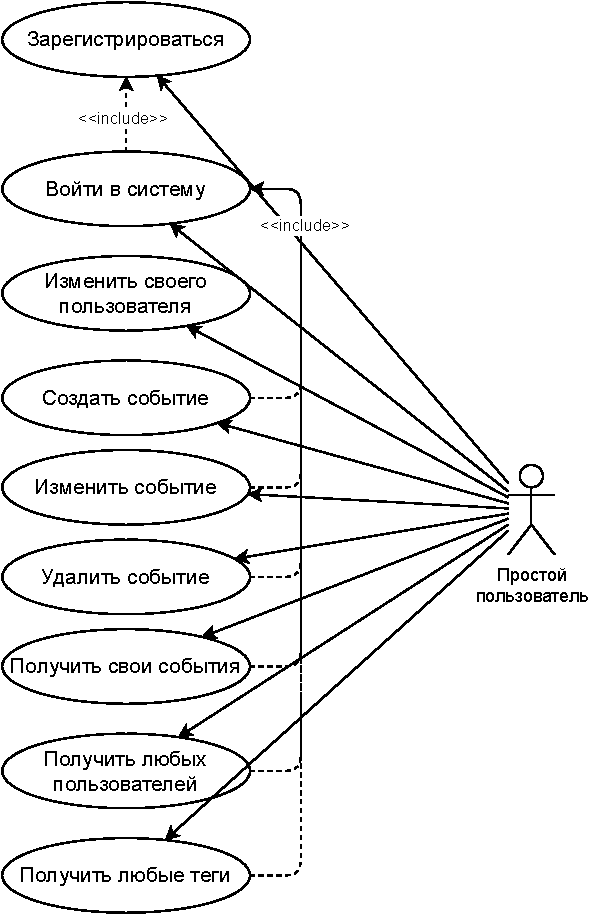
\includegraphics[width=0.9\linewidth]{assets/images/Use-Case-Простой.pdf}
	\caption{Use-case диаграмма простого пользователя}
	\label{fig:use-case-simple}
\end{figure}

\begin{figure}[ht!]
	\centering
	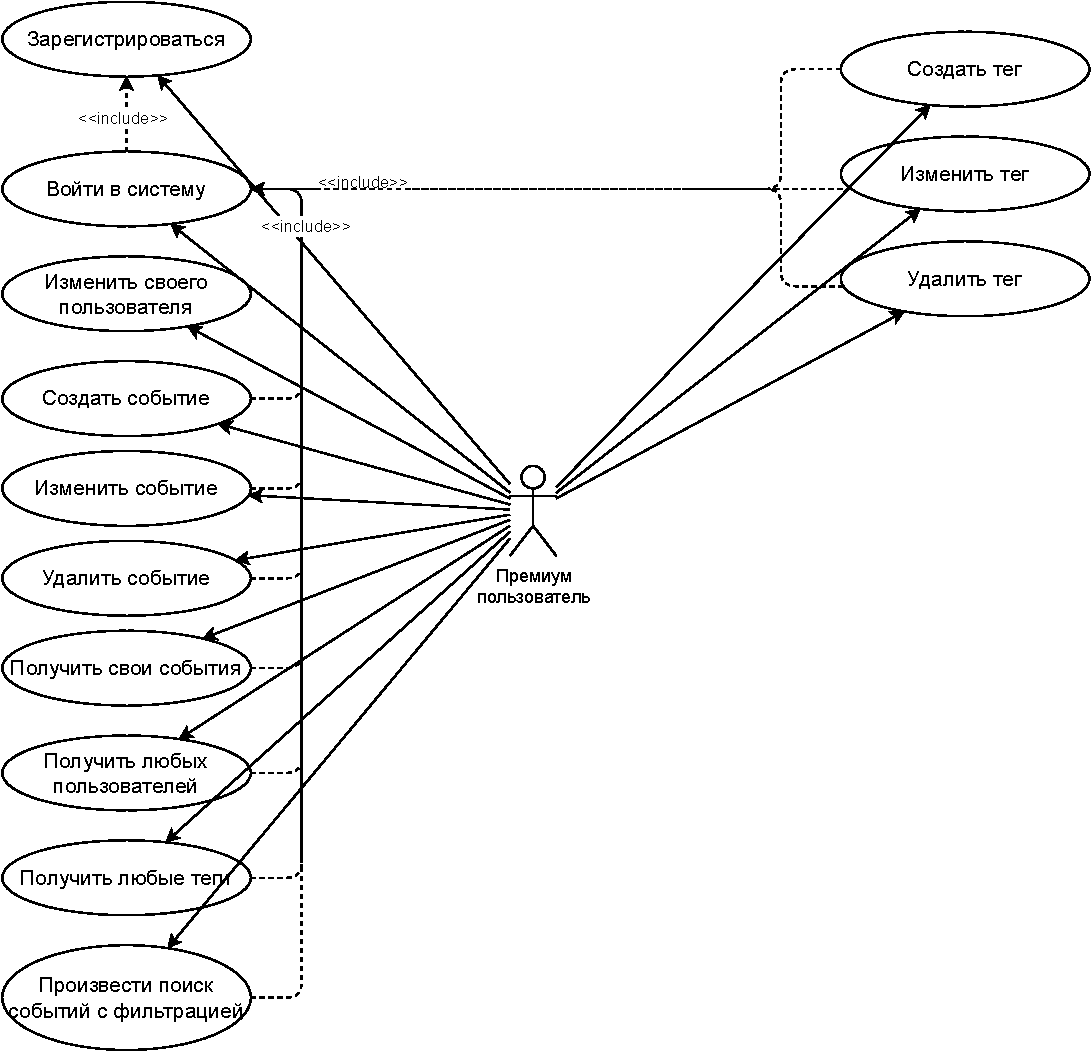
\includegraphics[width=0.9\linewidth]{assets/images/Use-Case-Премиум.pdf}
	\caption{Use-case диаграмма премиум пользователя}
	\label{fig:use-case-premium}
\end{figure}

\begin{figure}[ht!]
	\centering
	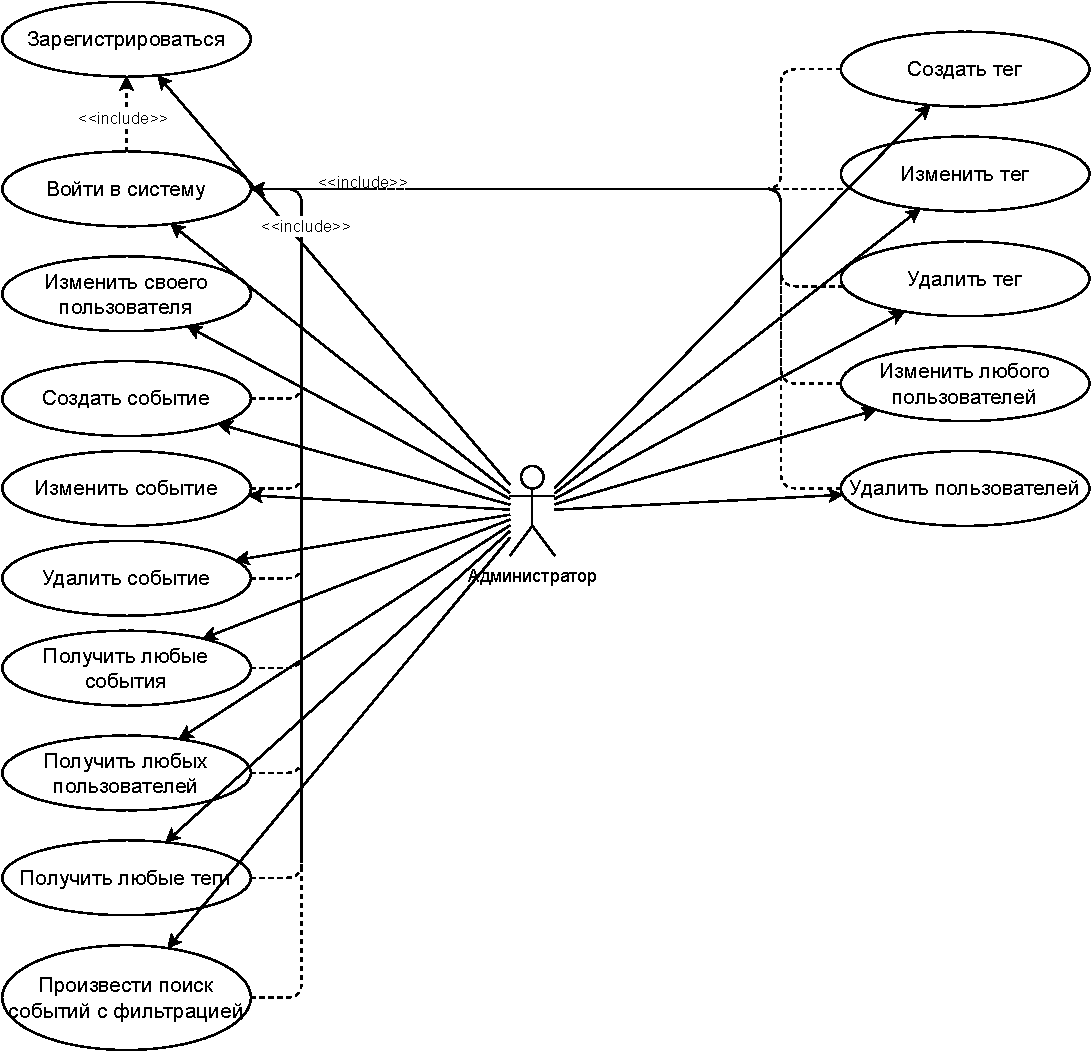
\includegraphics[width=0.9\linewidth]{assets/images/Use-Case-Администратор.pdf}
	\caption{Use-case диаграмма администратора}
	\label{fig:use-case-admin}
\end{figure}
\FloatBarrier


\subsection{Классификация СУБД}

Система управления базами данных, \textbf{СУБД} — совокупность программных и лингвистических средств общего или специального назначения, обеспечивающих управление созданием и использованием баз данных. Главные задачи СУБД – это создание базы данных и манипуляция данными. Такая система позволяет обеспечить надежность хранения данных, их целостность и неизбыточность.

Основными функциями СУБД считаются:
\begin{enumerate}[label=\arabic*.]
	\item управление данными во внешней памяти;
    \item управление данными в оперативной памяти с использованием дискового кэша;
	\item журнализация изменений, резервное копирование и восстановление базы данных после сбоев;
	\item поддержка языков БД.
\end{enumerate}

Классифицировать СУБД можно следующим образом:

\subsubsection{По модели хранения}

По модели хранения данных СУБД модно разделить на 3 категории:
\begin{enumerate}[label=\arabic*.]
	\item \textbf{Дореляционные}
		\begin{itemize}[]
			\item \textbf{Инвертированные списки} (файлы). БД на основе инвертированных списков представляет собой совокупность файлов, содержащих записи (таблиц). Для записей в файле определен некоторый порядок, диктуемый физической организацией данных. Для каждого файла может быть определено произвольное число других упорядочений на основании значений некоторых полей записей (инвертированных списков). Обычно для этого используются индексы. В такой модели данных отсутствуют ограничения целостности как таковые. Все ограничения на возможные экземпляры БД задаются теми программами, которые работают с БД. Одно из немногих ограничений, которое все-таки может присутствовать --- это ограничение, задаваемое уникальным индексом. 
			\item \textbf{Иерархическая модель} данных подразумевает что элементы, организованные в структуры, объединены иерархической или древовидной связью. В таком представлении родительский элемент может иметь несколько дочерних,
			а дочерний --- только один родительский.
			\item \textbf{Сетевые} --- могут быть представлены в виде графа; логика выборки зависит от физической организации данных.
		\end{itemize}
	\item \textbf{Реляционные} \cite{db_sql}
	
	В реляционных моделях данные организованы в набор двумерных взаимосвязанных таблиц. Каждая из которых представляет собой набор столбцов и строк, где столбец представляет атрибуты сущности, а строки представляют записи.
	Использование таблиц для хранения данных обеспечило простой и эффективный способ хранения структурированной информации, доступа к ней, а также легкую сортировку.
	
	\item \textbf{Постреляционные} \cite{db_nosql}
	
	Постреляционные базы данных реализуют схему с использованием нереляционной модели данных. Такие БД поддерживают логическую модель данных, ориентированную на обработку транзакций. 
	Постреляционные базы данных включают хранилища данных с ключевыми значениями, сетевые и графовые базы данных, а также базы данных, ориентированные на документы (например, поисковые системы).
	
	Недостатком такой модели является сложность решения проблемы обеспечения целостности и непротиворечивости хранимых данных.
\end{enumerate}

\subsubsection{По способу доступа к данным}

\begin{enumerate}[label=\arabic*.]
	\item \textbf{Файл-серверные} --- при работе с базой, данные отправляются приложению, которое с ней работает, вне зависимости от того, сколько их нужно. Все операции --- на стороне клиента. Файловый сервер периодически обновляется тем же клиентом.
	\item \textbf{Клиент-серверные} --- вся работа производится на сервере, по сети передаются результаты запросов, гораздо меньше информации. Обеспечивается безопасность данных, потому что все происходит на стороне сервера.
	\item \textbf{Встраиваемые} --- библиотека, которая позволяет унифицированным образом хранить большие объемы данных на локальной машине. Доступ к данным может происходить через SQL либо через особые функции СУБД. Встраиваемые СУБД быстрее обычных клиент-серверных и не требуют установки сервера, поэтому востребованы в локальном ПО, которое имеет дело с большими объемами данных.
	\item \textbf{Сервисно-ориентированные} --- БД является хранилищем сообщений, промежуточных состояний, метаинформации об очередях сообщений и сервисах;
	\item Прочие --- пространственная, временная и пространственно-временная.
\end{enumerate}


\subsubsection{Выбор модели базы данных}

В качестве основной для реализации данного курсового проекта была выбрана реляционная модель данных по следующим причинам:

\begin{itemize}[]
	\item задача предполагает постоянное добавление и изменение данных;
	\item задача предполагает быструю отзывчивость на запросы пользователя;
	\item задача предполагает надежное хранение данных.
\end{itemize}
 
Помимо этого, постановка задачи предполагает возможность осуществления быстрого поиска событий (с использованием фильтрации, сортировки и пагинации). Такой функционал предоставляют специализированные поисковые базы данных, относящиеся к классу постреляционных. Поэтому было принято решение использовать ElasticSearch для осуществления фильтрации, сортировки и пагинации событий в проектируемом приложении.

